% arara: xelatex
% arara: xelatex
% arara: xelatex


% options:
% thesis=B bachelor's thesis
% thesis=M master's thesis
% czech thesis in Czech language
% english thesis in English language
% hidelinks remove colour boxes around hyperlinks

\documentclass[thesis=B,english]{FITthesis}[2019/03/06]

%\usepackage[utf8]{inputenc} % LaTeX source encoded as UTF-8
% \usepackage[latin2]{inputenc} % LaTeX source encoded as ISO-8859-2
% \usepackage[cp1250]{inputenc} % LaTeX source encoded as Windows-1250

\usepackage{subfig} %subfigures
\usepackage{graphicx}

% \usepackage{amsmath} %advanced maths
% \usepackage{amssymb} %additional math symbols

\usepackage{dirtree} %directory tree visualisation

% % list of acronyms
% \usepackage[acronym,nonumberlist,toc,numberedsection=autolabel]{glossaries}
% \iflanguage{czech}{\renewcommand*{\acronymname}{Seznam pou{\v z}it{\' y}ch zkratek}}{}
% \makeglossaries

% % % % % % % % % % % % % % % % % % % % % % % % % % % % % % 
%%%%%%% CODE INSERTION START
%%%%%%%%%%%%%%%%%%%%%%%%%%%%%%%%%%%%%%%%%%%%
\usepackage{listings}
\renewcommand{\lstlistingname}{Source code}% Listing -> Source code
\usepackage{color}

\definecolor{dkgreen}{rgb}{0,0.6,0}
\definecolor{gray}{rgb}{0.5,0.5,0.5}
\definecolor{mauve}{rgb}{0.58,0,0.82}

\lstset{frame=single,
  language=Java,
  aboveskip=6mm,
  belowskip=0mm,
  abovecaptionskip=3pt,
  captionpos=b,
  showstringspaces=false,
  columns=flexible,
  basicstyle={\small\ttfamily},
  numbers=none,
  numberstyle=\tiny\color{gray},
  keywordstyle=\color{blue},
  commentstyle=\color{dkgreen},
  stringstyle=\color{mauve},
  breaklines=true,
  breakatwhitespace=true,
  tabsize=3
}

%%%%%%%%%%%%%%%%%%%%%%%%%%%%%
%%%%%%% CODE INSERTION FINISH
% % % % % % % % % % % % % % % % % % % % % % % % % % % % % % 

\department{Department of Software Engineering}
\title{Online Clearing center}
\authorGN{Mykyta} %author's given name/names
\authorFN{Boiko} %author's surname
\author{Mykyta Boiko} %author's name without academic degrees
\authorWithDegrees{Mykyta Boiko} %author's name with academic degrees
\supervisor{Ing. Stanislav Kuznetsov}

\abstractEN{The overriding objective of this thesis is dedicating to create a prototype of the web-application that would act as a marketplace connecting crypto-trades, investors and developers of trading strategies. It should help to monetise the work of cryptocurrency trading strategies developers and to maximise profit for crypto-traders and investors using trading "Buy/Sell" signals generated by trading strategies. Another equally important component of work is to provide REST API as to crypto-traders, investors as well to trading strategies developers and different tools helping with choosing the required trading strategy. Tools include candlestick chart describing price movement with the mapping of trading signals with already expired by that time validity, and statistical data giving an analysis of strategy performance based on measuring overall success or failure of signals predictions for every single strategy presented on the marketplace. The result should be a prototype of a future ambitious platform capable of creating competition in today's crypto trading market.}
\abstractCS{Hlavním cílem této práce je vytvořit prototyp webové aplikace, která by fungovala jako tržiště spojující krypto tradery, investory a vývojáře obchodních strategií. Mělo by to pomoct zpeněžit práci vývojářů kryptoměnových obchodních strategie a maximalizovat zisk pro krypto tradery a investory, kteří používají obchodní signály „Kup/Prodej“ generované obchodními strategiemi. Další neméně důležitou součástí práce je poskytování REST API jak pro krypto tradery, investory, tak pro vývojáře obchodních strategie a různé nástroje, které pomáhají při výběru požadované obchodní strategie. Nástroje zahrnují svíčkový graf popisující pohyb ceny s mapováním obchodních signálů s již vypršenou dobou platnosti a statistické data poskytující analýzu výkonu strategie založeného na měření celkového úspěchu nebo neúspěchu předpovědí signálů pro každou jednotlivou strategii prezentovanou na tržiště. Výsledkem by měl být prototyp budoucí ambiciózní platformy schopné vytvořit konkurenci na dnešním trhu krypto obchodování.}
\placeForDeclarationOfAuthenticity{Prague}
\keywordsCS{Kryptoměny, obchodní strategie, obchodní signaly, webová aplikace, PHP, Symfony, React JS}
\keywordsEN{Cryptocurrencies, trading strategies, trading signals, web-application, PHP, Symfony, React JS}
\declarationOfAuthenticityOption{1} %select as appropriate, according to the desired license (integer 1-6)
% \website{http://site.example/thesis} %optional thesis URL


\begin{document}

% \newacronym{CVUT}{{\v C}VUT}{{\v C}esk{\' e} vysok{\' e} u{\v c}en{\' i} technick{\' e} v Praze}
% \newacronym{FIT}{FIT}{Fakulta informa{\v c}n{\' i}ch technologi{\' i}}

\setsecnumdepth{part}
\chapter{Introduction}
Currently, cryptocurrencies are considered the most attractive alternative to conventional currencies. This is mainly confirmed by the absence of a regulator in the form of a central bank or government. Even with confidence, it can be argued, that they are guaranteed only by mathematics, and never by trust or people.
For both traders and ordinary people, cryptocurrencies are attractive due to massive investment potential, but at the same time, it is followed by a certain level of risk.

Over the past few years, the number of cryptocurrencies and platforms allowing exchange them has been enormously growing.  Considering that as opposed to traditional markets, cryptocurrency exchanges are never closed, that is tradings can be done at any time, the logical step of development was the emergence of various trading tools with a general principle of automated trading. Of the existing solutions, mainly can commonly identify three fundamental tools of automated trading. These are automated bots based on SaaS\footnotemark model, Robo-Advisors and scripts that can be executed in automatic or semi-automatic mode. Their purpose is to decrease or totally eliminate the human factor, thereby minimise the losses and maximise the profits. Mostly these are different software performing trades depending on predefined rules, in other words using trading strategies. Another existing solution is to use already created business strategies for a certain fee. These and other solutions will be described in more detail in the chapter “Analysis of existing solutions”.

\footnotetext{Software as a Service is a software delivery model or a cloud service, the gist of which is that software application is hosted on the internet or cloud and not on user environment.}

In the majority, trading strategies are the set of rules defining when a trader will take action and, typically, consisting of trade filters\footnotemark and triggers\footnotemark and typically including use of indicators or multiple indicators. Indicators are representing mathematically-based technical analysis tools used to analyse the past and predict future price trends. They provide trading signals required by strategy's triggers. A trade signal is a trigger for the action, either to buy or sell an asset. Existing various types of them, with manual or semi-automated execution based on market data, news and sentiment, besides, are used complex signals that are derived using existing signals.  

\addtocounter{footnote}{-2} %2=n
\stepcounter{footnote}\footnotetext{Set of criteria identifying the favourable conditions for entering market positions that the trader/investor most desires.}
\stepcounter{footnote}\footnotetext{It is any type of event that fulfils conditions to start an automated transaction without requiring any additional trader input.}

To date, solutions connecting traders and strategy developers provide various sets of services starting with trading signals or fully automated, not market depending, trading strategies, ending with low latency execution platform or even execution algorithms powered by Neural Networks and Genetic Algorithms. Of course, without forgetting to ensure security at all levels to all involved parties. Many platforms use their crypto coins as a means of payment.

However, no one should have any excessive illusions about all the above solutions. Any of them does not guarantee even something close to 100\% per cent success. Herein lies the significance of  “prediction paradox”:

\begin{quote}
"The more humility we have about our ability to make predictions, the more successful we can be in planning for the future."\cite{silver_signal_2015}
\end{quote}

The first and most relevant aspect which served as motivation for the appearance of this thesis was figuring out the absence of solution with open source code, that would offer the following:
\begin{itemize}
  \item adherence to the "mediator only" principle between two interested parties(all strategy implementation details is only on the developer's side).
  \item ensuring maximum security of all executed transactions, data transfers
  \item transparent visualisation
  \item timely, fast and safety delivery of signals to the destination, that is, the trader
  \item correctly designed API for both parties(developer and trader APIs)
  \item a notification system that will quickly alert the receipt of a new trading signal prediction
  \item payment system, similar to smart contracts\footnotemark(the developer will not receive the income before the contract is not fulfilled, a third party must approve the rightness of signal prediction)
  \item absolute extension ability(architecture that allows to add new features and expand the capabilities of old ones.)
\end{itemize}

\footnotetext{It is a program that controls the transfer of digital assets between parties based on the observance of certain conditions.}

The next just a little less important motivator was that no small part of implementation is Front-End development. For me, this is a kind of challenge. Almost all my programming experience falls to Back-End development. And at the same time, it is a good opportunity to get to know with web development modern technologies, deepen knowledge in the area of network communication, especially with ways of making them secure. Also, step to create a prototype of a trading platform, in connection of growing up trend to cryptocurrency, allows getting base knowledge in that area. Moreover,  it is a good practice for professional life, a project with real-world application.

The target audience for this product is both developers of signals that are provided by relevant strategy and any level of professionalism traders. Developers will be motivated by possibility not to trust the strategy implementation secrets to other parties and get stable, secure a platform for selling its services through a developer's API.
Traders, even in the case of a zero knowledge base, will be able to decide whether or not they want to use any particular strategy based on an analysis of the candlestick chart with mapped expired signals and based on the portfolio of strategy, namely statistics data that represent results of measuring strategy performance, profits and other indicators.

\section{Goal}
The whole bachelor thesis can be split into three major parts: Analysis, Design and Implementation, how it has to be in the RUP\footnotemark development process.

\footnotetext{Rational Unified Process is the software development process based on software engineering principles and commonly used to develop systems based on objects or component-based technologies.}

The goal of the research part is to grasp basic terms related to the content of the followed work, to analyse and explore already existed solutions based on established criteria. After the research part, as the next required components within the Analysis, are documented aspects of full production usage and basis for future expansions. It is also, the emphasis is placed on focusing more closely on the business processes around which the trading platform's prototype is built. Analysis part acts as the groundwork of followed work. 

Next logical step of work is Design part involved with such essential parts as preparing of database model, proposing a suitable architectural solution based on the results of the previous part. Also, there are provided other types of software design techniques for better representation of available functional possibilities related to proposed architecture. 

The Implementation part is devoted to a detailed step by step description of realisation itself. This chapter, on logical grounds, is divided to Back-End and Front-End parts. These both parts are preceded by a section from previous chapter, explaining the choice of any specific technologies. Here is also adduced information such as testing and user manual, relating to the already built and working prototype.

The last part of work, named Future Improvements, describes more thoroughly basis for future extensions that were already mentioned briefly in the Analysis chapter.

\setsecnumdepth{all}
\chapter{Analysis}
\section{The Theoretical Foundations}
This section provides a basic understanding of the key terms, whether they are new or just an extension of those already mentioned in previous chapters. They are necessary to cover every aspect of the subsequent work and, in particular, to contribute to the further theory building in the research section. Also, especially for the reader, it is necessary to get acquainted with them for a better understanding, and problem-free tracking of logical chains encountered in some parts of work.

First of all, are described terms which fill in the gaps in knowledge and leading up us to terms such as technical indicator, trading signal and its existed types are described. Next, are provided terms closely connected to them or structurally complementing the overall picture.

\subsection{Market}
It is a marketplace where goods, currencies, bonds and other assets are traded between two parties. Examples of such cryptocurrency markets are Binance, Poloniex, Bittrex, Bitfi-nex. The simplest example of classic trading is all known Forex.
\subsection{Market Pair}
Market pair or currency pair, it is a quotation of two different commodities (in the context of this work - cryptocurrencies) traded in markets. Currency pairs compare the value of one currency to another. First one is the base currency and the second is quote currency.
Placing an order for a currency pair works on the principle of buying a base currency when selling a currency quotation.
\subsection{Candlestick Chart}
The candlestick represents aggregated information about the price of two commodities in a pair over a certain period (1 minute, 1 hour or 1 month).  One or more candlesticks, in turn, form a candlestick chart. Every single candlestick contains the four most significant values, as it can be seen in the diagram \ref{fig:OHLC}. (And that is sort of why it is technically called OHLC):
\begin{figure}[!ht]
\centering
\caption{OHLC Chart}
\subfloat{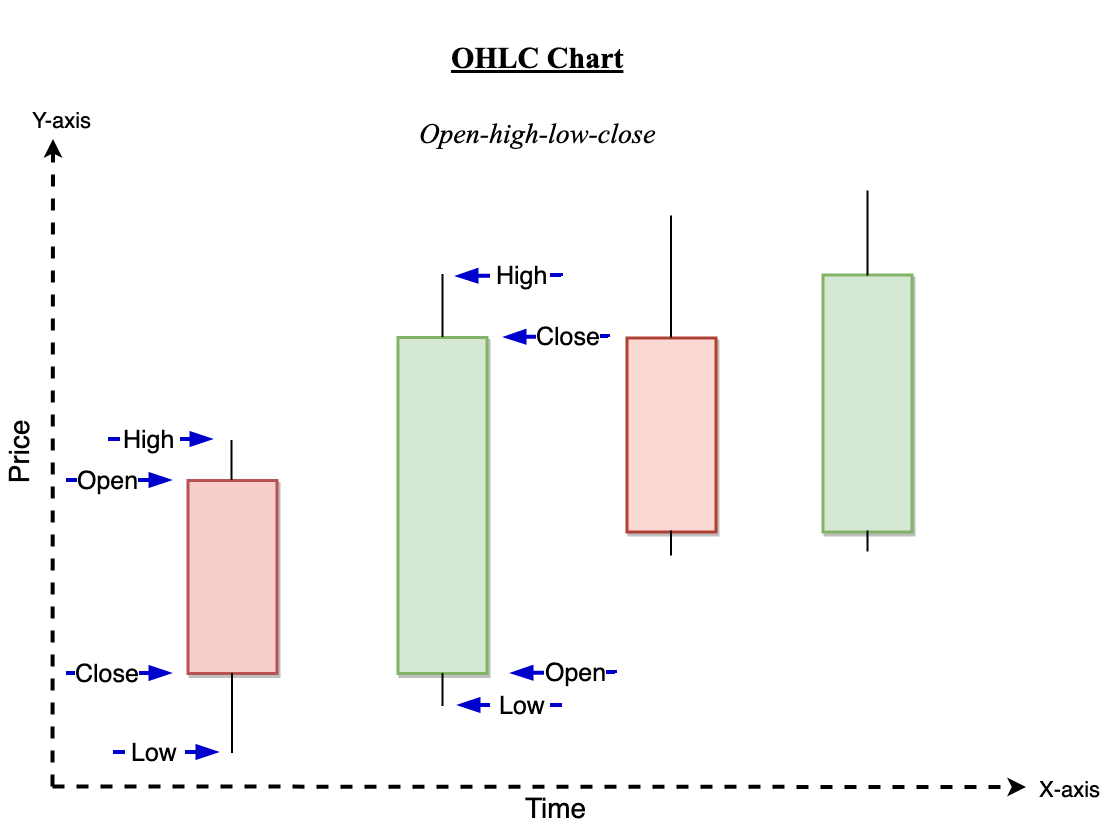
\includegraphics[width=0.8\columnwidth]{figures/OHLC_Chart}}
\label{fig:OHLC}
\end{figure}

\begin{itemize}
\item
\textit{Open} - price value at the beginning of the period.
\item
\textit{High} - value of maximum price in the period.
\item
\textit{Low} - value of minimum price in the period.
\item
\textit{Close} - price value at the end of the period.
\end{itemize}

\subsection{Indicators}
It is important to note at the outset that an indicator is not a trading strategy. Indicators are statistics used, first of all, to measure current conditions and secondly to predict either financial or economic nature trends. 
Indicators, commonly, are divided into economic indicators and technical indicators.
\begin{itemize}
\item 
\textbf{Economic indicators}. Economic indicators are a part of economic data on a macroeconomic scale, submitted in the form of statistical metrics. They are used by analysts in order to interpret current or future possibilities for investors.

\item 
\textbf{Technical indicators}. In the context of technical analysis, one should begin with the fact that technical trading involves the examination of charts and taking the decision based on patterns and indicators.
These patterns in question, are specific shapes that candlesticks form on a chart. They may contain information about the price future direction. The application of any technical indicator to the chart adds to the overlays, which contain additional information through mathematical calculations of price and volume. These transformations are used to predict future price and volume information.

Technical indicators, in simple terms, are mathematical calculations that are displayed on the chart.

Common technical analysis indicators are the moving average convergence-divergence, abbreviated as MACD indicator and RSI indicator, short for relative strength index.
\end{itemize}

\subsection{Cryptocurrency Indices}
A crypto index is a trading asset whose base is based on several crypto pairs of leaders in the digital market segment. It is a really good source of information for activities such as comparative analysis, monitoring and most importantly, comparison of growth of different cryptocurrency assets. Crypto indexes allow traders to invest safely in almost the entire currency market.
Creation of own high-quality index is kind of a difficult job. It is justified by the fact that it derived from a number of parameters including price, market cap, and past performance etc. And in principle, the larger the data sample, the better accurate it will be in tracking the whole market.  And furthermore, the ideal cryptocurrency index consists of every single coin in the market, in addition, they are weighted by market cap. But it does not change the fact that crypto index is a good source of information helping in keeping your finger on the pulse in the cryptocurrency world.


\subsection{Trading Signals}
In plain language, trading signals are trade suggestions, or simple alerts, or, to be more precise, triggers for action which determines if there needs to buy or sell a particular coin under certain conditions such as specific price, time and others. There exists a huge variety of signals type and below are provided most popular of them, depending on the type of analysis they are based by.
\begin{itemize}
\item 
\textbf{Technical signals}. In most cases,  the technical analysis, generated by any kind of technical indicators, is a major component using in a signal generating. It should also be noted that technical analysis is the study of past market data to predict the direction of future price movements. Technical patterns are considered to be good predictors for identification of entry and exit points in trading. 


\item 
\textbf{Sentiment signals}. Alternative data is the term that can be applied to datasets outside of financial, economic indicators and, to be more precise, it refers to a subset of big data used in ML\footnotemark \footnotetext{Machine learning is a type of algorithms that allows improving accuracy in outcomes predictions of software applications due to automatic learning, gained experience and without much intervention in the programming part.} and improving algorithms. They are increasingly used in traditional markets filled with players and strategies in order to find an advantage. The most simple example of "alternative data" in cryptocurrency is social media sentiment.

Today it has long been known about the existence of solid relationships between cryptocurrency price movement and content of social media. Sentiment analysis is an application of ML where consistently performing the process consisting of information aggregation, data analysing and trends determination in price and sentiment. Sentiment signals are generated as the output of ML performing. Because of that, news and sentiment play a rather important role in signals sources in trading.  


Based on the data used to derive sentiment, the most common subtypes of sentimental signals are listed below:


\begin{itemize}
\item
\textbf{News-based signals}. News flow serves as important sources of signals in trading. The main challenge is that occur non-uniform and not structured news data sources, and there is a lot of it and directly from this flows difficulty in understanding whether the news is perceived by the market as positive or negative, whether the story content is new or just recycled by someone.

Mainly,  when creating news-based signals, the analysis of the news itself is carried out by utilising various NLP\footnotemark \footnotetext{Neuro-Linguistic Programming is a modeling approach that offers techniques of exploring the relationship between communication, thinking and behaviour and techniques to improve communication, change behaviour and achieve goals.} and ML. An interpretation of story content following that and, just in much less than a few seconds, after the news is published, is created the “buy” or “sale” alert. 
 

Summarising the above information, the news-based signals are high-frequency tools seek to track the various types of events spread through the news, to understand their meaning using predefined algorithms and, finally, to predict the likely direction of price movement that can be caused directly by these events.
It stems from the fact that they can influence the prices of crypto assets.

\item
\textbf{Social-based signals}. Next type of non-trivial sentiment signals is social signals and its derived almost exclusively from social media sources like Twitter, Telegram, Reddit, Bitcointalk and others. Analysing the relationship between the discussion around certain cryptocurrency in the social media or, to be precise, the emotional state of the cryptocurrency community and the price of its asset may be used to create trading signals.  Unfortunately, performing of such monotonous and time-consuming work like reading the daily news on Bitcoin, this cannot be done efficiently by a single person or even by the team – this is the type of job that can be handled only by AI\footnotemark. \footnotetext{Artificial intelligence makes it possible for machines to simulate the human intelligence processes and to perform human-like tasks. Returning to NLP, simply, it is the part of AI but strongly connected to processing the human language, usually written.} 

Mostly, social-based signals are based on measuring such factors as quantity (quantity of tweets),  quality (positive or negative sentiment) and velocity (ratio of quantity to time) of sentiment data or even combination of them.

\end{itemize}

\item
\textbf{On-chain data-based signals}. These trading signals based on the analysis of the blockchain data. To their creation, the well-tested techniques are employing, used for market data analysis in the traditional markets. Depending on the angle at which to look on blockchain data, there are two main types can be distinguished.

The first type mainly explores various metrics of the on-chain transactions and as well as the creation of a wallet. The process involves cleaning data from noise and setting statistical relationships,  which in turn have considerable predictive power.

The second type deals with really large type transactions and known wallets movements using the principle of on-chain data mapping.  The core of principle is mapping the on-chain space by identifying exchange wallets, storages and other on-chain actors and creating of algorithmic models based on significant on-chain movements or transactions.

This type of trading signals is especially useful in combination with the social sentiment data on a specific asset.
\end{itemize}
At the prototype design level, only technical signals are used. In subsequent chapters, in order to avoid difficulties, only the term trading signals will be used, by which we mean precisely signals of a technical nature.

\subsection{Algorithmic Trading System}
The term "algorithmic trading" could be explained as something like using a computer program to automate any number of steps you need in the trading process. The definition is rather vague. Besides, it is rather difficult to explain, but in fact, it is not particularly interesting to us. However, here is something that really should interest us is the architecture of the algorithmic trading system.

Algorithmic trading systems consist of much more than only trading strategies. They may consist of several components, each of them is responsible for a specific trading process aspect. The fundamental components of it are the data, pre-trade analysis, trading signal generation, trade execution and post-trade analysis.  A more detailed introduction to the structure and relationships between the components is shown in the diagram \ref{fig:CATS}. Some components may be missing, and vice versa, some additional components may be present.

The first component is Research, and it does not require special attention from us. More accurately, it can be labelled as Research systems, and in short,  it involves a mix of interactive development and fully automated scripting. 

The second one is a Data component that is basic to the entire system, and it can interact with the rest of the system as well it is used by every single component of it. This component fundamentally is a staging area for the various data received from external sources such as market, non-market, current or historical sources, with following resending of them for pre­processing and, therefore preparing for the analysis. Pre­processing involves in the first step is filtering out the irrelevant data to avoid possible noise capable of the negative effect the strategy used. The second step is extraction of filtered data, transformation them into a standard format and loading them to the end target. Also, based on pre­defined business rules, is being ensured the integrity of that data. It should be added that as data, also, can be used news, tweets and data from social media.

At the level of Pre-trade analysis component, data of such types as crypto, financial and semantic, are used to predict trends, thereby helping to decide where to send orders and exactly when, whether to use algorithms or trade an order manually. Some of the techniques used to get a market prediction including the various analyses types among which, for example, known well to us, technical analysis. Also, the analysis of data can be logical split up into alpha (prediction of future financial instruments behaviour), risk (evaluation of the financial instruments risk level) and transaction cost (calculation of potential costs associated with the same financial instruments) models.  There is no sense in describing the purpose of each model. For a general understanding, it is enough already said above.

The Trading signal generation component may be easily confused with the component of the Pre-trade analysis or the Trade execution. However, speaking of its essence, this component mainly uses information accumulated from the pre-trade analysis with following applying of other different technical analysis techniques using market data to achieve the defined goal. Typically this included goals such as whether the profits maximisation or developing an entry and exit strategy and others. Moreover, continuing with the theme of similarity to components above-specified, it gives us more detailed, concretised information and, also, the taken decisions can lead to possible trades. The result of component performing is a trading signal indicating when to buy or sell a particular asset. Well, anyway, another important factor is that this component can be a part of a trading strategy.

Also, we should quickly go through the remaining components, which in the framework of the development of the prototype we should not be particularly interested in. 

The Trade execution layer is responsible for making decisions based on which performed routing of orders to the market, simply put, it is an order execution strategy. Based on received data from previous components, component read market conditions and create relevant orders.

The Post-trade analysis component must obtain feedback from results of algorithm interaction with the market and include it to the application, for example, for future possible control measures.

In summary, it can be said that the trading process itself could be separated into three stages: trading signal generation, trading decision, and trade execution. An analysis of the architecture was carried out in order to define in a certain sense the boundaries of the prototype being created. 

The trading system to be created, the designations in the task, should approximately correspond, with possible changes of some components, the architecture shown, but, mainly, excluding of the components of the Trade execution and Post-Trade analysis. Do not forget that most of all we are interested in everything related to trading signals.

\begin{figure}[!ht]
\centering
\caption{Components of an Algorithmic Trading System}
\subfloat{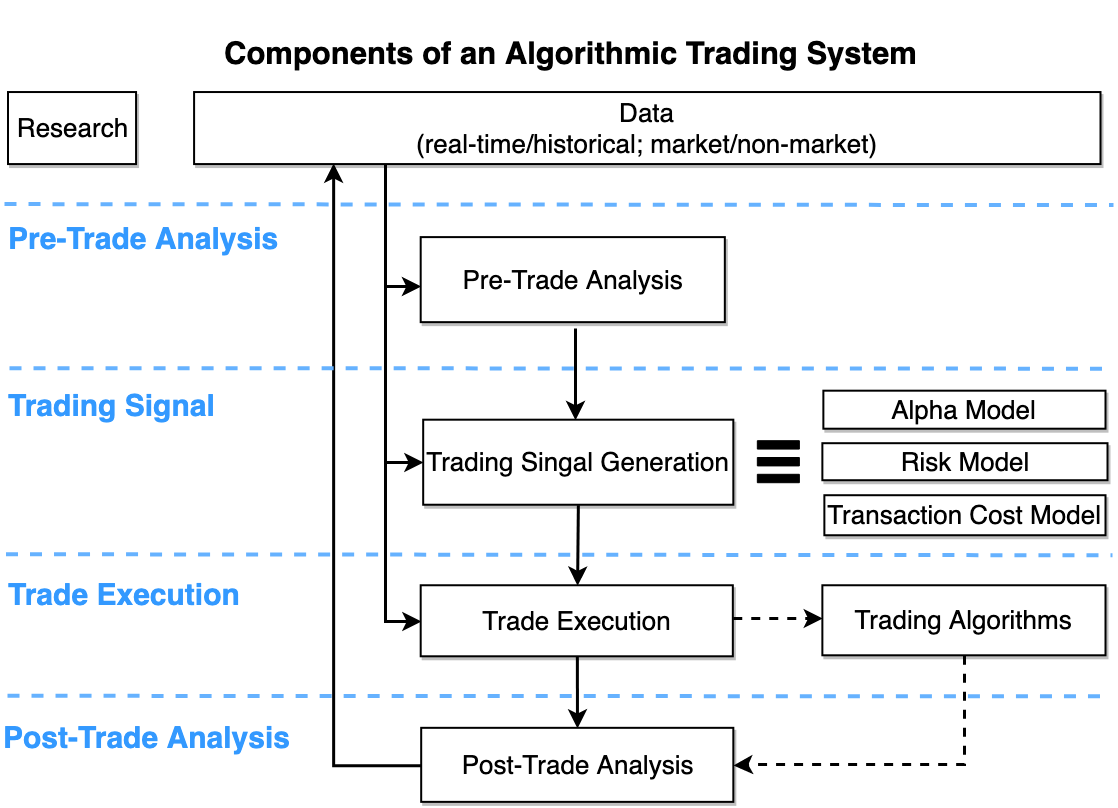
\includegraphics[width=0.8\columnwidth]{figures/CATS}}
\label{fig:CATS}
\end{figure}

\section{Research of existing solutions}
This section contains a list of existing solutions and a brief analysis of their functionalities. The goal of the bachelor's work goal strongly identifies that the prototype must be in the form of web-application. Therefore, regarding technical aspects, we consider solutions that only web-based functioning, ignoring any software that requires forced installation on a local PC.

Unfortunately, the overwhelming majority of existing solutions fall into paid and closed segment. The required open-source solutions are not presented in the public domain so far, let alone solutions that are close in logical-semantic aspects or similar in the functional-structural base. At the same time, this is logical enough that in an area where there is sufficient cash flow, all restrictions and standards are also fully complied with, including implementation secrets.

Therefore, in conclusion of the above, this is by no means a surprise for us and, conversely, logically narrows the range of solutions under consideration to the segment of commercially closed solutions.

Before the search for existing solutions, should go back a few steps, where it is necessary to clearly define the model of the expected search results and properties it should have.
The modern market offers us platforms with varying degrees of automation. For example, it can be an assisted type trading system that allows a trader to manually confirm an order before sending it to the exchange or system can be fully automated, which means that it does not require any type of activity from the trader and can freely send orders to the exchanges.

Let consider existing solutions in the form of trading platform of different levels of automation, but the only thing, reverting to the diagram \ref{fig:CATS}, the main thing that we need is implemented component Trading signal generation. Ideally, solutions that maximise the emphasis on selling/buying trading signals. Naturally, with the ensuing features, for example, notifying the trader about receiving a trading signal in the form of alerts. Also, the implementation of components that are placed on the diagram above the Trading signal generation component will not be superfluous. Moreover, a crucial moment is the presence of the API for both parties, as for traders as well for developers. The minimum framework is established and, finally, now it is possible to start considering existing solutions.

\subsection{Commercially closed solutions}

\addtocontents{toc}{\protect\setcounter{tocdepth}{2}}
\subsubsection{Crypto Hopper \cite{noauthor_cryptohopper_nodate}}
Cryptohopper is cryptocurrency trading bot hosted in the cloud, founded in July 2017. It is a web-based solution with a friendly, clear user interface, and it has a cloud-like infrastructure. The bot is easily managed from any web browser and works around the clock. However, it was noticed that sometimes trading bot's performing slows down due to the time of high traffic on the website. 

The platform is hosted on Amazon Web Services, and its servers are secured by them. Regarding security, the website is protected by a firewall and active protection against DDoS, which provides the company Cloudflare. All sensitive data are encrypted in the database stored on the server. Besides, exists the possibility to activate two-factor authentication(2FA), its default turned off. 

As for the functional part, the platform has its marketplace, where can be found trading strategies templates and trading signals developed by other traders. The ability to create a trading strategy based on custom parameters, from scratch is also available. Moreover, the platform uses a subscription model, that is, every trader can subscribe to any trading strategies and signals from, whether platform approved or third-party sellers.

Just in time for what has been said above about the presence of signals in the marketplace,  should also be added about such an exciting feature as the integration of professional external signals, named Signals/signalers, that should remind us of social trading elements. Signals are input data for the bot, just adjusting its trading behaviour. Signaller is a service that is run by people to scan the crypto markets, and to look for signs of an upward move. Signallers commonly use cloud computing and  ML algorithms for viewing a large number of technical indicators for cryptocurrencies. Every trader can apply to become a signaler. All it requires is to fill the appropriate form including such details as a subscription fee, social platforms and motivation. It needs to wait for approve from administrators and only after that we will get the signalers membership. It should be noted here that this is not such an easy and quick process.

To the word, as such, a notification system alerting about the received new trading signal is missing. The only thing that "Last Signal Output" tab is presented in the dashboard, that, according to name, shows last received signals. A trader is probably unlikely to know about the received signal without opening the dashboard page. It seems to be severe enough omission.

The trader is required to provide API keys to the bot, which using them will make trades on exchanges. The exchanges generate these API keys, and transferring them to the bot will give it only restricted access to the trader's account for trading purposes.

\subsubsection{MetaTrader 5 \cite{noauthor_metatrader_nodate}}
Meta Trader 5 represents an electronic widely used trading platform and is simultaneously trading software. This software is consists of server and client components and provided by MetaQuotes Software. 

However, in truth, we are more interested in the web-based solution,  the search for which leads us to the MetaTrader 5 Web Platform, more precisely, to a separate component named WebTrader.
Fundamentally, this is just a web version containing all the standard usability and is fully compatibility with the entire MetaTrader 5 ecosystem and no additional software.

Regarding security, all the connections that are used for data exchanges between the system components and, also, all system databases are highly encrypted. Besides, built-in advanced systems such as authentication and authorisation, provide accounts protection.

The platform uses the MQL5 language allowing to perform a variety of functions such as tracking financial symbols around the clock, analysing and others. MQL5 is a high-level OOP language based on C ++ and specialising in solving various trading tasks, developed by MetaQuotes Software.

The Market tab leads us to the world's largest secure store of various trading tools provided with such representational data as graphs, descriptions and other. Such trading tools as bots, trading strategies, indicators, scripts are presented. Almost every trading solution in this market can be bought, rented or, moreover, every doubter can test a demo version of a decision helping to make a final decision.

To assume the seller role in a MetaTrader Market needs to complete a standard registration form with specifying of contact data. Before publishing in the Market, every program is appropriately tested.

Furthermore, close to the Market tab, the Signals tab can be found. It represents Trading Signals service or, more precisely, copy trading service.  That does not speak about providing trading signals in the common understanding of the word. In truth, it works as that the trader provides public access in the form of a subscription to the deals that he executes in the market.  During a valid subscription, received signals are automatically executed on trading accounts of subscribers. In the same way, as it was said above about sellers of trading tools in the Market, everyone can become a provider of signals.

Also, an important fact is the ability to test trading strategies against historical data provided by the platform and to apply different optimisation techniques.

\subsubsection{Zignaly}
Zignaly is a platform for trading by whether bot or manually. Regarding the first variant, the entire platform can be defined more precisely, namely, Zignaly is a signal bot. Its functional capabilities are almost limited with just reacting to incoming signals. This said it must be noted that the platform is still in the development process and to date, the only we can analyse is the beta version of the future ambitious extended platform.

It is a web-based cloud platform with a secure environment, where traders can trade 24 hours connecting to preferred signal providers. They can accept trading signals, with following using them, whether based on their own rules or relying on auto-mode. Also, the opportunity to create our signal provider is available. It can have both public and private access types, depending on the needs of the provider. The public access type requires sending some signals directly to the platform administration in order to check for the presence of bad ones. Signal providers are given the choice of how to deliver individual signals. Whether by email or directly to the endpoint.

To set a new trading strategy with a full set of relevant built-in functional capabilities in the form in which we know it, Zignaly integrates the TradingView\footnotemark service, which allows using various indicators designed for this purpose or, as an alternative, to use the internal trading terminal of the platform. 

\footnotetext{TradingView is a cloud-based charting and social-networking software, where traders can share information about changes in the e-money market as well as the securities market.}

Regarding security and, in particular, access rights to the assets of an individual trader, the Zignaly platform does not have such rights.
Continuing on the subject, digital assets are stored on individual crypto exchanges and rights to withdraw them are not provided to platform.

One of the main features against the background of the other similar platforms is transparency provided by the trading bot. Every trader that uses bot can easily communicate with the platform developers in case of needs.

Besides, among the platform's underlying advantages is that there is no coins limit for trading with the platform. There is no need in selecting coin pairs, just because all the pairs enabled by signal providers are accepted by the platform.

\section{Business Modeling}
The main object of this section is to create the first layer of the software development lifecycle. Besides, this layer will be a key to understanding system requirements and as well as for identification of system use-cases.
Among advantages of generating web-application prototype can be highlighted generating different visions, understanding of technical feasibility and others.
The most crucial step at this stage is to understand how to create a usable web-application by analysing user requirements.
So when we look at a detail of this section, we have to cover the basic overview of the business, that is, business processes, products and stakeholders which are required for application development.

\subsection{Concept}
'Online Clearing center' is an upcoming web-based online trading platform or, put simply, a marketplace to sell trading signals targeting the traders and investors living all around the world. The suppliers of those trading signals are different trading strategies taken their places in our marketplace. They are provided by developers and require a paid subscription form, in that way developers monetise the use of their product by the second party. Each developer is free to set subscription fee of any amount and traders, in turn, must pay for each signal received during an active subscription, using funds in an e-wallet. 

To make things easier for our potential clients and, at the same time, move with the times, are introducing such independent, external component as auditors. Auditors play supervisory, sometimes, a regulatory role in the transaction system of the upcoming marketplace. Mostly, they are responsible for tracking the fulfilment of the terms of the order contract. Which gets us to the point that until all the order conditions are fulfilled - the funds will not reach the service provider’s e-wallet, but will simply be frozen.

All kinds of activities, including business transactions, have to be only through the online marketplace. 

\subsection{Products}
Online Clearing center will sell trading signals, and at the prototype level, they are limited only by a subgroup called technical signals. The trading signal represents a kind of advice for traders in the form of predicted movement direction in the market, or in other words, whether is better to buy, sell or hold assets at the designated time interval and at what cost — this information identified by an understandable set of data contained in the trading signal itself.

Since the underlying idea of the upcoming online market is that almost everything revolves around trading signals and all related processes, it seems quite logical to create a system that allows to instantly and at the same time quite intuitively transfer trading signals to traders with an active subscription. 
 
\subsection{Stakeholders}
Traders,  investors, trading strategies developers, automated trading bots and auditors are the primary stakeholders for Online Clearing center business.

\subsubsection*{Traders}
A trader is an individual that engaged in dealing with buying and selling of assets in any market, in our case, cryptocurrency market. He does it, either for himself or on behalf of another person or institution.  A trader can be highly skilled or with zero knowledge, but he is interested in the platform where he can find a variety of different trading strategies, select prefered one a start to receive predictions about different market pairs. Based on this, it is safe to make final decisions or to deepen knowledge in the field of market analysis.

\subsubsection*{Investors}
An investor is any person or entity who allocates funds to grow them by receiving returns. An investor typically is different from a trader. The difference lies in the period of obtaining the expected profit. For an investor, the objective is that it is long-term gain. Any investor can be interested in our marketplace, seeing it as an aggregator of different solutions helping to predict the future market in form trading signals. With the help of them, an investor can build a huge analytic base for solving long-term profit-oriented objectives.

\subsubsection*{Trading strategies developers}
Trading strategy developer is a person with the use of different analysis techniques, in our case, technical analysis, able to create an automated solution to predict market behaviour in the form of trading signals and, mainly, want safely monetise his product without providing to any other parties secrets of implementation.

\subsubsection*{Automated trading bots}
An automated trading bot is a tool for automated trading in any or defined market. It includes a set of predefined rules and, mostly, based on the event-driven model. That is means that it expects events, an example can be a trading signal, that should trigger it and, depending on whether the conditions are met, trading operations will be conducted.  Typically, it can collect more than one trading signal and as a result of comparing them, possibly with using more additionals analysis layers such as applying of in-built filters, conduct trading deals. Our marketplace platform can be interested in terms of an easily accessible source of such triggers.  

\subsubsection*{Auditors}
An auditor is an individual or a firm that is responsible for evaluating the validity of accounting data belonging to a particular organisation.
As part of our platform, the duties of the auditor will include validating the correctness of the prediction of the trading signal or in other words, investigating the difference between actual and predicted values looking for any unusual results. For this purpose are used historical data from the relevant exchanges, analytical base, and so on. 
Based on the result of the performed investigation, an auditor makes a report which involves either, in case of bad prediction, returning of frozen funds to payers or in case of good, transferring all funds to destination e-wallet excluding platform usage commission.


\subsection{Business processes}
Next crucial step is to take a look at key business processes describing stakeholder expectations. Expanding the definition, business processes, are chains of activities that performs user with a particular purpose using application. Identifying of them is a crucial part of development that helps better understand work subject, highlight key system parts (on which is needed to focus more) and not the least to recognise potentially problematic parts in time. For visualisation business processes in our application's boundaries is used UML (Unified  Modeling  Language) activity diagrams created in \textit{Enterprise Architect} program.

As mentioned above, only key business processes will be listed. It is because the selected compilation is sufficient to cover the main ideas, and even if absolutely everything was listed without exception, this would be an unnecessary additional work due to the lack of new, useful information.

\subsubsection{Registration of new trader/developer}
The primary and fundamental to all other processes is the registration process. It all starts with the transition of an unregistered user to the main page of the web application. Where the initial step is to fill in the registration form. In case of a problem with filling in, the user will be informed what the reason: incorrect/not-unique/bad parameters. In another case, he will be informed about the successful creation of his profile and, also, instructed to go to the mailbox specified in the registration form, to confirm the own account, which, is currently unverified.

In his mailbox, the user must find a welcome mail from the platform with a confirmation link containing a unique identification key. It is generated immediately during filling in the registration form and, currently, it serves to identify the user only unverified account.

This key has a certain expiration date for security purposes. After the expiration of the term, all manipulations with it should come to nothing. The only thing that the user will be to repeat the entire registration process from the very beginning.

If the key is still valid, then, using this link would be confirmed the user's account and displayed the login page.
Finally, all, that will be left for the user is to fill in the authentication form with a followed automated system login. Only the registered users with the verified account could pass authentication. 
Besides, at that step ends the registration process.

\subsubsection{Adding a trading strategy to the marketplace}
Process of adding a new trading strategy to the marketplace, in fact, precedes the primary web-application process, which is, subscribing to preferred trading strategy or strategies with next receiving of trading signals. The process itself includes a simple sequence of steps, but with its nuances. Therefore, it is worth giving a few words to this. For a better understanding of the following description will be accompanied by a diagram \ref{fig:BP_ADD} from which we can superficially get acquainted with the process, without deepening into the details.
Most things are clear when looking at a diagram. It is not clear, for example, that among the required fields in strategy creation form are such things as the choice of an exchange market and a cryptocurrency pair, the corresponding strategy works with them. 
Besides, after success adding strategy to our marketplace, the developer gets the unique identification key, called the API key, that will use according to platform rules. The existence of such key allows us the to correctly identify the developer and, also, relevant trading strategy, when is started data flow from developer's side whether in the form of the trading signals transferring or other data types.

\begin{figure}[!ht]
\centering
\caption{Business process of adding a trading strategy to the marketplace}
\subfloat{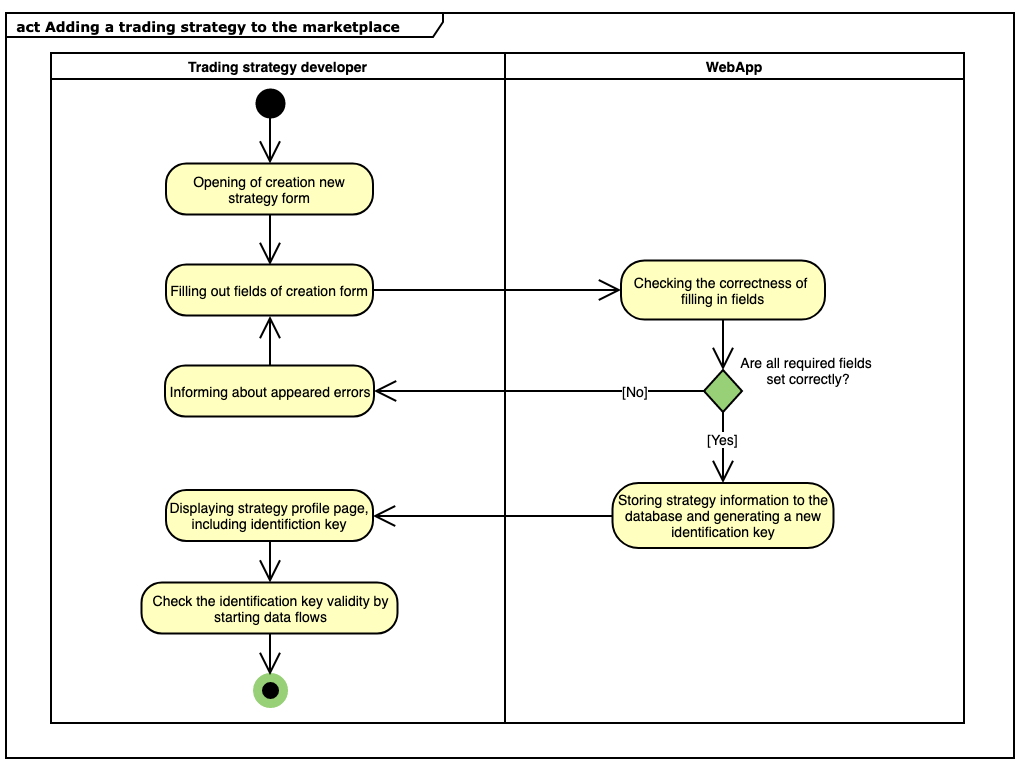
\includegraphics[width=0.9\columnwidth]{figures/activity_adding_strategy}}
\label{fig:BP_ADD}
\end{figure}

\section{Requirements analysis}

\subsection{Functional requirements}

\textit{Functional requirements describe the services the system should provide. Sometimes the functional requirements state what the system should not do. Functional requirements can be high-level and general or detailed, expressing inputs, outputs, exceptions, and so on.} \cite[p.~47--48]{laplante} \\

\noindent \textbf{F1: Market signals} \label{f:1}

\noindent The main functional requirement is that the platform provides a way of buying and selling cryptocurrency market signals. \\

\noindent \textbf{F2: Strategies statistics} \label{f:2}

\noindent The platform provides clients with information about strategy statistic, based on which they can predict the profit from money investment to some strategy. Traders are able to decide whether or not to use any particular strategy based on an analysis of the candlestick chart. \\

\noindent \textbf{F3: Notifications} \label{f:3}

\noindent The platform has a notification system that will quickly alert the receipt of a new trading
signal prediction.\\

\noindent \textbf{F4: Payment system} \label{f:4}

\noindent The main purpose of the platform is to provide a meeting place for traders and developers of trading strategies. We provide payment system, similar to smart contracts, which ensures each payment. The contract should be fulfilled to transfer funds to the developer. \\

\noindent \textbf{F5: Log} \label{f:5}

\noindent In case of error during the workflow, the platform will provide users with meaningful messages. \\

\subsection{Non-functional requirements}

\textit{Non-functional requirements are imposed by the environment in which the system is to exist. These requirements could include timing constraints, quality properties, standard adherence, programming languages to be used, compliance with laws, and so on.} \cite[p.~47--48]{laplante} \\

\noindent \textbf{NF1: Performance and stability} \label{nf:1}

\noindent The platform should work in a reasonable timeframe because signals have a limited lifetime. We are responsible for providing actual data to traders. Also we have to ensure server stability. Otherwise we have to pay all possible losses.\\

\noindent \textbf{NF2: Security} \label{nf:2}

\noindent We provide a highly secured platform for strategies trading. Developers want to keep secret implementations of their strategies and at the same moment, have a apportunity to sell it without fear. Ensuring maximum security of all executed transactions, data transfers. \\

\noindent \textbf{NF3: Extensibility} \label{nf:3}

\noindent Platform architecture supports trouble-free future extension in case of need, due to huge potential of creating competition in today’s crypto trading market. \\



\chapter{Design}
\section{Used technologies}
The choice of used technologies has been derived from goals set in the previous chapter. The whole application was divided into Back-end and Front-end parts. It is very suitable for separating application logic from user interface and visualization. 
This step gives us separation of responsibilities and thus covering reducing components complexity.
Back-End, mostly, is responsible for resource management, downloading of data and its persistence.
Regarding Front-End, it is, mostly,  providing a user interface that guarantees marketplace quick access, grabs traders attention and don't give a chance to get lost using alert system that is spread all through the application.
Communication between two layers, Back-End and Front-End, is performing in way of realisation of API service by Back-End.


\subsection{ReactJS} 
 ReactJS is an open-source JavaScript library for building user interfaces. The building blocks of any user interfaces created with ReactJS are components. They are typically written using JSX --  an extension to the JavaScript language syntax similar to XML.  

 \subsection{Redux} 
As a library for developing user interfaces, ReactJS is often used in combination with other libraries, such as Redux, for example.
Redux is a predictable state container for ReactJS.  
There is a far easier way to explain it in a few words. It can be imagined as a big object that owns and operates with almost every piece of data are needed by an application on the client side to function.
It should be said for deepening understanding, that Redux is founded on three described principles below, so:
\begin{enumerate}
 \item \textit{Single source of truth} - there is one, and only one place which represents the state of the entire application.
 \item \textit{State is read-only} - it is simply mean, that it can be only changed by the action.
 \item\textit{Changes are made with pure functions.}
\end{enumerate} 

\subsection{Symfony 4}
Symfony is an open source PHP framework that simplifies the process of developing a web application. 
The framework is fast develops, has extensive documentation of many extensions. Framework Components are a set of the reusable PHP libraries, namely covering such aspects as object configuration, routing, authentication, templating and many more.
Any of these components can be easily installed with the PHP dependency manager, which is known to almost everyone and this is Composer.

For working with a database, the Symfony framework uses a Doctrine ORM.
However, to avoid undue questions, below is the list of a kinda the advantages why to use Symfony exactly in combination of Doctrine:
\begin{itemize}
	\item Supports annotations, XML and YAML for schema.
    \item Uses DQL (Doctrine Query Language) that that provides truly extended querying capabilities over the object model.
    \item Doctrine keeps data consistent by performing perform cascade actions and using foreign keys.
    \item Doctrine forces the developer to disengage from holding inside head any such data as, for example, table field names and instead of that uses repository pattern.
\end{itemize}



\subsection{Communication protocol}
Another fundamental step leading us to the creation of a future working prototype is communication protocol between backend and frontend. HTTP protocol was chosen for communication between Back-End and Front-End. Because the goal of the work is to implement a platform that allows real-time visualisation of trading strategy predictions results, in our case that is trading signals, there was a need to find suitable technology that allows really quick and efficient communication. According to different network sources knowledge basements, the choice fell on  Web Application Messaging Protocol.

\subsubsection{Web Application Messaging Protocol}
Real-time messaging between server components and the client could be implemented using the Web Application Messaging Protocol.  For Symfony framework exists solution --  ThruwayBundle, which is a PHP implementation of WAMP. 
 


\section{Deployment Model}
The deployment model represents a relation between software and physical hardware when the application is running. 
The model is presented in figure \ref{fig:BP_DEPLOYMENT}. There are three physical nodes depicted: 
\begin{enumerate}
 \item client 
 \item client's server 
 \item application server
\end{enumerate}
First two nodes communicate with the server through two different communication protocols: HTTP and WebSocket.  
 \begin{figure}[h]
\centering 
\subfloat{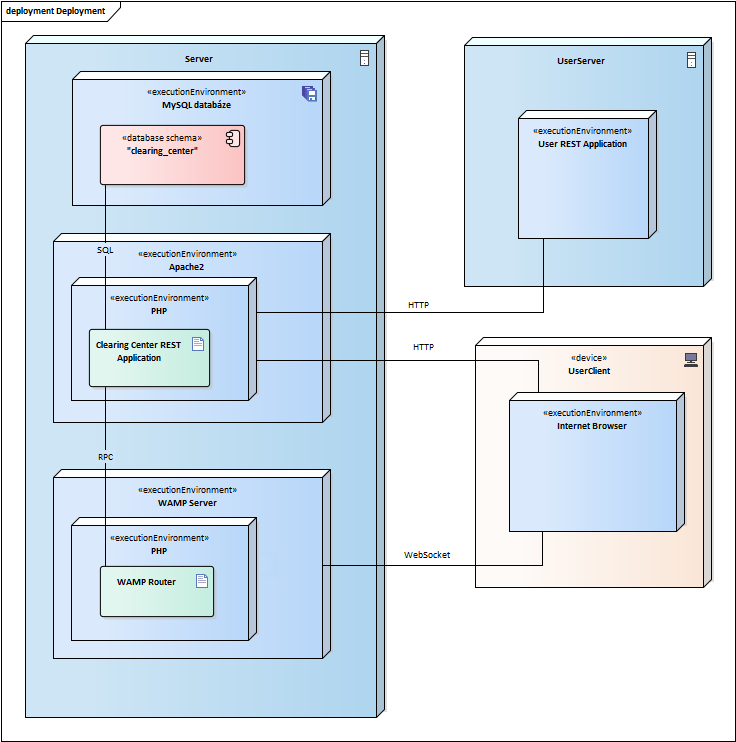
\includegraphics[width=1\columnwidth]{figures/deployment}}
\caption{Deployment diagram} 
\label{fig:BP_DEPLOYMENT}  
\end{figure}  



\section{Architecture}
Based on the deployment model, the system is developed based on the client-server architecture, where the server implemented as a Web server and the client presented in two types: 
\begin{enumerate}
 \item Web application
 \item Remote server
\end{enumerate} 
Communication between the server and the client is carried out using the REST API.  An interactive connection additionally used between the server and the Web application using Web Sockets technology.
Given the above, the entire application divided into two modules: Back-end and Front-end. The architecture of the whole application captured in figure \ref{fig:BP_ARCHITECTURE}.
 \begin{figure}[!ht]
\centering 
\subfloat{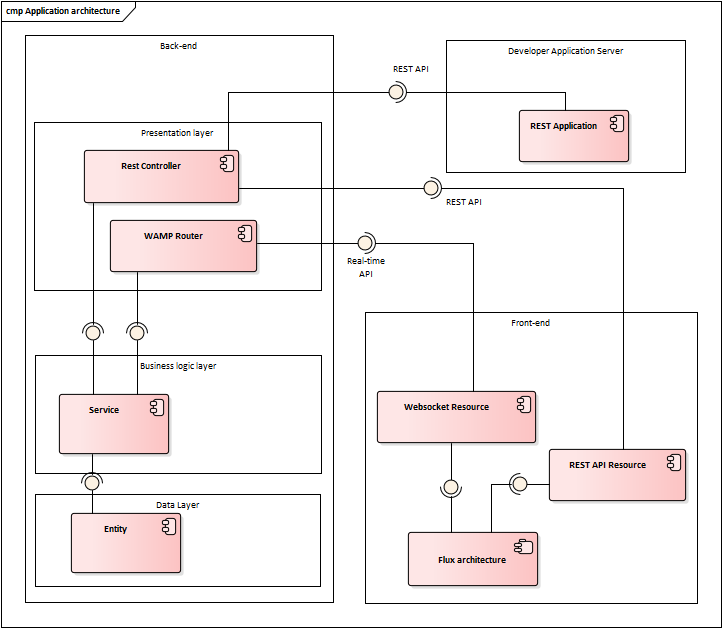
\includegraphics[width=1\columnwidth]{figures/architecture}}
\caption{Application architecture}
\label{fig:BP_ARCHITECTURE} 
\end{figure} 
\subsection{Back-end} 
This module divided according to a three-tier architecture, which divides the application into three tiers: presentation tier, application tier and data tier.  Separation of these tiers will allow more flexible changes and more natural development of reusable components.
\subsubsection{Entity}
Entities represent objects located in the Application. They contain their definition, access methods, and specify how a particular class should map to tables within the database. 
\subsubsection{Services}
Services are responsible for processing the received data and   drives an application's core capabilities
\subsubsection{Rest Controllers}
Rest Controllers represent the endpoints for accessing the Application through the Rest API. They are used only for incoming and outgoing requests and use the respective Services for any more demanding operations. Those controllers are part of the presentation layer (although it only presents data in JSON format).
\subsubsection{WAMP Router}
WAMP Router represents the rest of the application's presentation layer.   Services publish messages for WAMP Router, and router distributes it to all subscribers.
 
\subsection{Front-end} 
The web application designed as a single page application. Single Page Application is an application that runs in the browser and does not reload the page during operation. 
ReactJS supports the Flux architecture. By this architecture, the module divided into four main components:  
\begin{enumerate} 
\item Store - holds the application state
\item Dispatcher-  specify how the action transforms the state
\item View - react components that grab the state from Store
\item  Action -   helps to facilitate passing data to the Dispatcher
\end{enumerate}
Figure \ref{fig:BP_FLUX_ARCHITECTURE} shows, how data flows between these components.
So, the main feature of the Flux-architecture is one-way data flow. This approach helps to make the code more predictable. 
 \begin{figure}[!ht]
\centering 
\subfloat{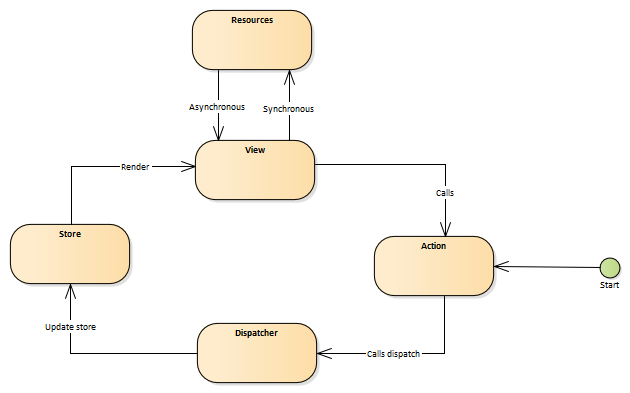
\includegraphics[width=0.8\columnwidth]{figures/flux_architecture}}
\caption{Flux architecture}
\label{fig:BP_FLUX_ARCHITECTURE}  
\end{figure}  
\section{Database}
 \begin{figure}[!ht]
\centering 
\subfloat{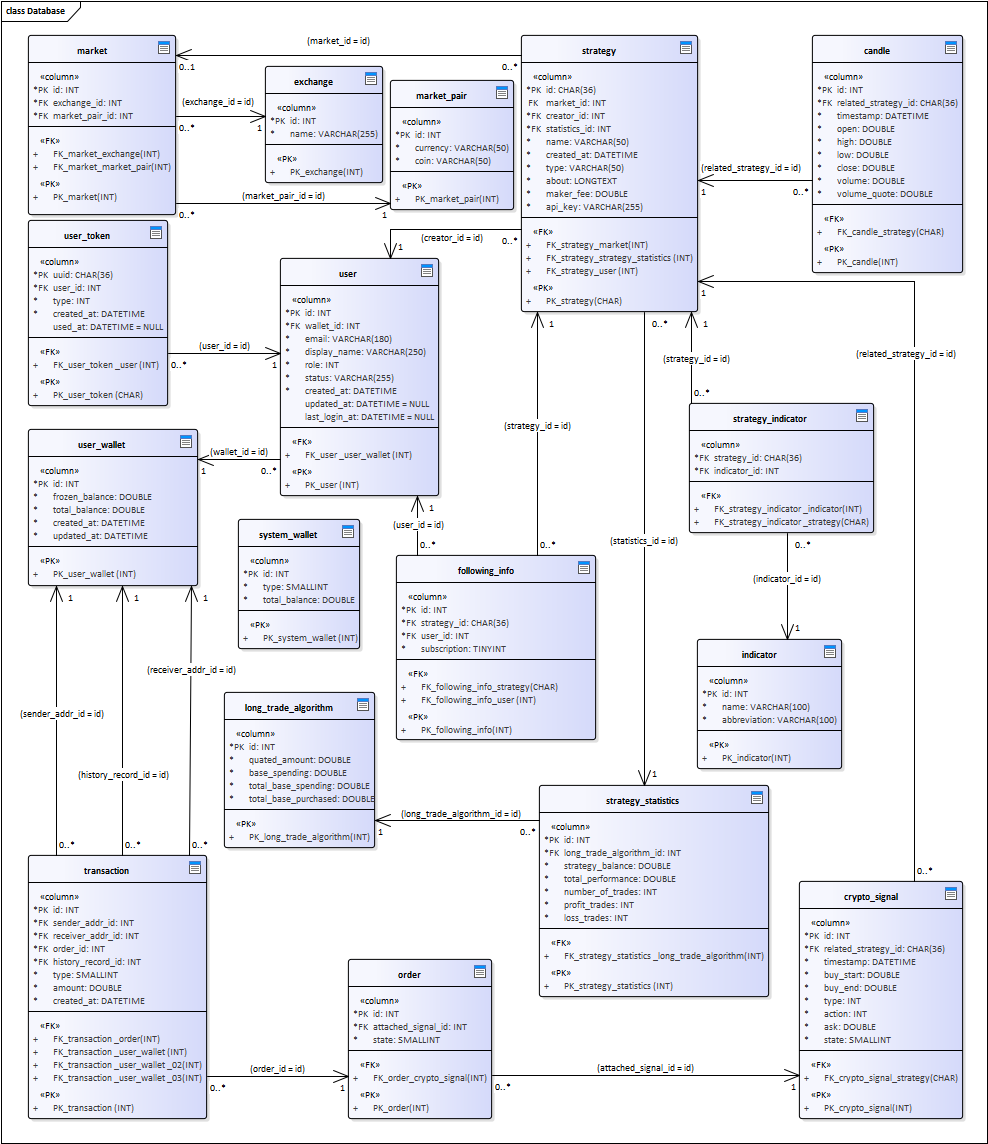
\includegraphics[width=1\columnwidth]{figures/database}}
\caption{Database} 
\label{fig:BP_DATABASE}   
\end{figure}   
\chapter{Realisation}
  
\section{Implementation}
The implementation part of the thesis divided into two logical parts according to the architecture design: back-end and front-end. This section covers the essential parts of the development.
\subsection{Back-end}

\subsection{Technology stack}
The platform's Back-End was implemented in PHP7.3 programming language.

\subsection{Dependency manager}
PHP composer was used to manage dependencies.
File composer.lock is kida of .gitignore file.
When you deploy dependencies to an application during development, the Verfile.lock file locks. It is distributed along with the application.
 
\subsection{Front-end}
Front-end implementation  passed in several stages: 

\begin{itemize}
  \item Creating project structure

According to the application architecture,  was created following the structure of the application:
    - views - contains React components
    - reducers, middleware, and store represent Store component in Flux architecture
    - styles and shared  
    - assets - contains styles, images, and other static files
    - actions represent an Action component in Flux architecture
    - constants 
    - helpers 
    - app   
  
  \item Creating of presentational component 
  
  Presentation components have only one responsibility to render HTML. In other words, presentational components are concerned with the look. These components fit for their elements creation. For better understanding, in listing 3.1 given a simple code of using Presentational Component pattern. The code generates a clickable button. But, if in quality of buttonName was set to empty line, the button will not be generated. In this way, immediately in all places, where this function will be called, the check will be performed.  

\begin{lstlisting}[float, caption=Source code of the Button function, label=code:button]
function Button(props) {
  return   <button type="button"  
            disabled={props.onClick === ""}
            onClick={props.onClick}>
          {props.buttonName}
        </button>;
}
\end{lstlisting}

In this phase, the following custom elements were implemented:
button, table, input, tabs, card, grid, spinner, alert, notification, navigation, sidebar, and footer. 
   
  \item Creating of Redux components

    At this stage, on the Back-end side were created all necessary REST API endpoints, which return MockUp data. Therefore, it became possible to create basic Redux components: Actions and Reducers.
    
    Example of Action is shown on listing 3.2. Example of Reducer is shown on listing bellow.
    
    
  
\begin{lstlisting}[float, caption=Source code of the nameReducer function, label=code:nameReducer]
  const initialState = {
    name: "Button"
  }

  function nameReducer(state = initialState, action) {
    switch (action.type) {
      case REDUX\_SET\_NAME:
        return {
          ...state
          name: action.name,
        } 
    }
  }
\end{lstlisting}  
  
  \item Creating Container Components and their introduction into Redux architecture
  
Unlike presentational, container components are connected to external objects. They might wrap several presentational components, and they might interface with Redux. In other words,  container components are concerned with making elements work.

Example using Container Components as View is shown on listing bellow. 


\begin{lstlisting}[float, caption=Part of the ContainerComponent class source code, label=code:ContainerComponent]
class ContainerComponent extends React.Component { 
    render() { 
    }
}

const mapStateToProps = (store, props) => ({
  ...state
});

const mapDispatchToProps = dispatch => ({
  removeName(): () => dispatch(setName("")) 
});

export default connect(mapStateToProps, mapDispatchToProps)(ContainerComponent);
\end{lstlisting} 
  
  \item Creating an HTTP connection and his introduction into Redux architecture
  
    For creation HTTP connection was used Javascript library Axios. 
    Example of asynchronous request using Action 

\begin{lstlisting}[float, caption=The source code of the create function, label=code:create]
export function create (values) { 
  return (dispatch) => {
   dispatch({type: CREATE});
   axios.post('/url', values)   
    .then((res) =>{
      dispatch({type: CREATE\_SUCCESS});
    })
    .catch((error)=> {
      dispatch({type: CREATE\_FAILURE});
    })
  }

}
\end{lstlisting}

CREATE, CREATE\_SUCCESS, and  CREATE\_FAILURE types must be added to Reducer.     
  
  \item Creating a WebSocket connection and his introduction into Redux architecture
  
      For creation WebSocket connection was used Javascript library Wampy. 
    To embed this type of connection into Redux architecture necessary to use Redux middleware.
    A middleware is a higher-order function that composes a dispatch function to return a new dispatch function. It often turns async actions into actions.
  
\end{itemize}

\section{Testing} 
An essential part of the development is testing the implemented solution. Testing is performed using Unit tests.
This type of tests is focused on the functionality of the classes in isolation. The Symfony Framework integrates with a PHP library named The PHPUnit Testing Framework.

Unit tests are targeted at Service's classes. The application does not have complete code coverage. Such an approach would be too time-consuming, considering the scope of the code.
 

\setsecnumdepth{part}
\chapter{Conclusion}
From begging the aim of the work was to design and implement a prototype of a future a trading platform that in most cases have to behave as a marketplace connecting trading strategies developers and, interested in their prediction solutions, traders. From begging development stages, was definitely clear on early development stages, that at prototype level as development process as well ready product is highly limited by different aspects not depending on us to date. Lack of a more less theoretical base, any kind of experience in the cryptocurrency world.
But, finishing with parts not depending on us, the goal of bachelor thesis and all the points of the assignment were fulfilled.

Based on a huge analysis part and following investigation a secure platform for trading. The functionality of the resulting application has been experimentally verified.

The various tools provide every new trader with the various type of data that helping him to make a decision if it needs to subscribe or is enough only follow a particular trading strategy. Thus, each trading strategy is fully characterized by its own profile page with candlesticks charts highly describing its performance in the market for last n-selected days or statistical data that is the result of simulation trading algorithm. All this data have the purpose to give now, at least a  future profile page structure view, and to define the ground to future possible extends and improvements.

This work was a real challenge, but a great benefit to me. I have improved my knowledge of understanding basic cryptocurrency world terms, principles of market predictions, exchange markets itself and gained practical experience with PHP and ReactJS in the context of this project. 

The potential for further development is enormous. The first natural step should be the involvement of the module responsible for communication with stock exchanges. It was a really good idea to increase performance involving new technologies, also, among trading strategies in the marketplace add other prediction solutions, especially with a different type of automatisation and maybe with other types of market orientation.
Finally, should be implemented as a strategy builder tool in the form of a built-in platform module for best performance and the greatest possibilities for an audience.

\bibliographystyle{iso690}
\bibliography{mybibliographyfile}

\setsecnumdepth{all}
\appendix

\chapter{Acronyms}
% \printglossaries
\begin{description}
	\item[GUI] Graphical user interface
	\item[XML] Extensible markup language
\end{description}


\chapter{Contents of CD}\label{app:CDcontent}

\begin{figure}
  \dirtree{%
    .1 readme.txt\DTcomment{the file with CD contents description}.
    .1 src\DTcomment{the directory of source codes}.
    .2 platform\DTcomment{the directory of platform source code}.
    .2 thesis\DTcomment{the directory of \LaTeX{} source codes of the thesis}.
    .3 figures\DTcomment{the thesis figures directory}.
    .3 *.tex\DTcomment{the \LaTeX{} source code files of the thesis}.
    .1 text\DTcomment{the thesis text directory}.
    .2 thesis.pdf\DTcomment{the Bachelor thesis in PDF format}.
  }
\end{figure}


\end{document}
